\chapter{Schrittl"angensteuerung\label{chapter:thema}}
\lhead{Schrittl"angensteuerung}
\begin{refsection}
\chapterauthor{Pascal Horat und Matthias Kn"opfel}
\printbibliography[heading=subbibliography]

\section{Problemstellung}
\rhead{Problemstellung}

Beim numerischen L"osen eines Anfangswertproblems (Kapitel \ref{chapter:numerik}) wird die L"osungskurve schrittweise berechnet.
Dabei wird ein Wert $y(t)$ auf dieser Kurve aus dem vorangegangenen Wert $y(t-h)$ ermittelt.  

Ist der zeitliche Unterschied $h$ zwischen dem vorangegangenen und dem aktuellen Wert zu gross, kann das bei engen Kurven zu grossen Fehlern f"uhren.
Diese Fehler k"onnen sich nun von Schritt zu Schritt fortpflanzen, sodass die L"osungskurve schlussendlich keine "Ahnlichkeit mit der exakten Kurve zeigt.
Als Konsequenz kann nun einfach der zeitliche Unterschied $h$, die Schrittl"ange, kleiner gew"ahlt werden.
Somit wird der Fehler pro berechnetem Wert kleiner und darum die L"osungskurve genauer.
Dies hat aber zur Folge, dass viel mehr Werte berechnet werden m"ussen, was mehr Rechenaufwand mit sich bringt.
So wird vor allem auf Kurvenabschnitten mit geringer Richtungs"anderung unn"otig Rechenzeit verschwendet.

Das Ziel dieser Arbeit ist nun, verschiedene Methoden zu entwerfen, welche die Schrittl"ange je nach Gegebenheit anpassen k"onnen. 
Die entwickelten Methoden werden an einem Beispielproblem getestet und nach vorbestimmten Kriterien untereinander verglichen.

\section{Beispiel}
\rhead{Beispiel}

Um die Schrittl"angenproblematik zu erl"autern, wird ein geeignetes Beispiel ben"otigt, welches folgende Anforderung erf"ullt: 
\begin{itemize}
\item Die L"osung sollte \glqq lange gerade Strecken\grqq~und Stellen mit grossen "Anderungen beinhalten, damit die Algorithmen an ihre Grenzen stossen.
\item Das Problem sollte schnell und leicht verst"andlich sein, denn in diesem Kapitel geht es schliesslich um die Schrittl"angensteuerung.
\item Das Konzept der Schrittl"angensteuerung und dessen Vorteile sollten damit auf einfache Weise visualisiert werden k"onnen.
\end{itemize}
Auf Grund dieser Voraussetzungen wurde als Beispielproblem das allgemein bekannte \em Zweik"orperproblem\em~gew"ahlt.
Bei diesem Problem geht es darum, das Verhalten zweier K"orper, welche ohne "aussere Einfl"usse miteinander wechselwirken, zu berechnen. 
Die Berechnungen werden zur Vereinfachung nach den Gesetzen und Axiomen von Newton vorgenommen, das heisst die relativistischen Effekte gem"ass Einstein werden ausser Acht gelassen.
Ausserdem wird von Massepunkten ausgegangen.
Damit gilt nach dem Newtonschen Gravitionsgesetz folgende Gleichung:
\begin{equation} \label{eq:newton}
F_1 = F_2=\frac{G m_1 m_2}{r^2}
\end{equation}
In obiger Formel ist $G$ die universelle Gravitationskonstante und $r$ der Abstand zwischen den beiden Massenpunkten.
Eine weitere Vereinfachung bringt die Annahme, dass beide Massen gleich sind. 
Damit erfahren beide K"orper vom Betrag her die selbe Momentanbeschleunigung $a$.
\begin{equation}
F=\frac{G m^2}{r^2}=m a
\end{equation}
Auf die momentane Beschleunigung umgeformt gilt somit:
\begin{equation}
a=\frac{G m}{r^2} \label{eq:beschleunigungSkalar}
\end{equation}
F"ur die weitere Betrachtung ist es sinnvoll in mehreren Dimensionen zu rechnen.
Aus diesem Grund wird die Formel nun aufgewertet.
Jeder K"orper $K_i$ hat eine bestimmte Position welche durch seinen Ortsvektor $\vec{s_i}$ beschrieben wird.
Der Abstand zwischen zwei K"orpern $K_1$ und $K_2$ ist damit die Differenz der beiden Ortsvektoren  $\vec{s_1}$ und $\vec{s_2}$:
\begin{equation} \label{eq:abstand}
\vec{r_{12}}= \vec{s_2}-\vec{s_1}
\end{equation}
Die Gleichung (\ref{eq:beschleunigungSkalar}) sieht in Vektorschreibweise umgeformt also folgendermassen aus:
\begin{equation} \label{eq:gravitationVektor}
\vec{a_1} =\frac{G m}{\mid \vec{r_{12}}\mid ^2}\cdot \frac{\vec{r_{12}}}{\mid \vec{r_{12}}\mid}=  \frac{d^2 \vec{s_1}}{dt^2}
\end{equation}
Der Ausdruck $\frac{\vec{r_{12}}}{\mid \vec{r_{12}}\mid}$ hat die L"ange $1$ und bewirkt das $\vec{a_1}$ in Richtung des K"orpers $K_2$ zeigt.
Ausserdem ist die Momentanbeschleunigung bekanntermassen die zweite Ableitung des Weges. 
Das Problem wird weiter vereinfacht, indem die beiden K"orper symmetrisch zum Ursprung angeordnet werden und sich wegen der gleichen Masse auch symmetrisch bewegen.
Somit sind die beiden Ortsvektoren $s_1$ und $s_2$ antiparallel:
\begin{equation}
\vec{s_2}=-\vec{s_1}
\end{equation}
Die Gleichung (\ref{eq:abstand}) reduziert sich damit auf:
\begin{equation}
\vec{r_{12}}= -2\vec{s_1}
\end{equation}
Dies hat wiederum Auswirkungen auf Gleichung (\ref{eq:gravitationVektor}):
\begin{equation}
\frac{d^2 \vec{s_1}}{dt^2} =\frac{G m}{\mid -2\vec{s_{1}}\mid ^2}\cdot \frac{-2\vec{s_{1}}}{\mid -2\vec{s_{1}}\mid}
\end{equation}
In dieser Gleichung kommen jetzt nur Gr"ossen vor, welche im Zusammenhang mit dem K"orper $K_1$ stehen.
Damit reicht es, wenn nur das Verhalten von einem K"orper untersucht wird. 
Darum k"onnen auch die Indizes weggelassen werden.
\begin{equation}
\frac{d^2\vec{s}}{dt^2}=\frac{G m}{4\mid\vec{s}\mid ^2}\cdot\frac{-\vec{s}}{\mid\vec{s}\mid}=-\frac{G m}{4\mid\vec{s}\mid ^3}{\vec{s}}
\end{equation}
Nun wird das Ganze in Komponentenschreibweise ausgedr"uckt.
Um das Problem "ubersichtlicher zu gestalten, wird es auf zwei Dimensionen beschr"ankt.
\begin{equation}
\frac{d^2}{dt^2}
\begin{pmatrix}
s_x \\ s_y
\end{pmatrix}
=
-\frac{G m}{4(s_x^2 + s_y^2)^\frac32}
\begin{pmatrix}
s_x \\ s_y
\end{pmatrix}
\end{equation}
Weil $\vec{s}$ auf der rechten Seite nur mit einem Skalar multipliziert wird und beim Ableiten eines Vektors jede Komponente einzeln abgeleitet wird, kann die Gleichung aufgeteilt werden.
Damit ergibt sich folgendes Gleichungssystem zweiter Ordnung:
\begin{equation} \label{eq:kompSchreibwEins}
\frac{d^2s_x}{dt^2}=-\frac{G m s_x}{4(s_x^2 + s_y^2)^\frac32}
\end{equation}
\begin{equation} \label{eq:kompSchreibwZwei}
\frac{d^2s_y}{dt^2}=-\frac{G m s_y}{4(s_x^2 + s_y^2)^\frac32}
\end{equation}
Um die L"osung der Differentialgleichung mit bestimmten Anfangsbedingungen zu berechnen, muss diese in einem bestimmten Format dem L"osungsalgorithmus "ubergeben werden.
In diesem Fall wird das Mathematikprogramm MATLAB verwendet. 
"Ubliche Solver in MATLAB verlangen Differentialgleichungssysteme mit Differentialgleichungen erster Ordnung.
Aus diesem Grund muss die Ordnung der beiden Gleichungen (\ref{eq:kompSchreibwEins}) und (\ref{eq:kompSchreibwZwei}) reduziert werden. 
\begin{equation}
\frac{d}{dt} \begin{pmatrix}
s_x \\ 
s_{x1}\\
\end{pmatrix} = \begin{pmatrix}
s_{x1} \\ 
-\frac{G m s_x}{4(s_x^2 + s_y^2)^\frac32} \\
\end{pmatrix}
\end{equation}
\begin{equation}
\frac{d}{dt} \begin{pmatrix}
s_y \\ 
s_{y1}\\
\end{pmatrix} = \begin{pmatrix}
s_{y1} \\ 
-\frac{G m s_y}{4(s_x^2 + s_y^2)^\frac32} \\
\end{pmatrix}
\end{equation}
Zusammengesetzt ergibt sich folgendes Differentialgleichungssystem:
\begin{equation}
\frac{d}{dt} \begin{pmatrix}
s_x \\ 
s_y \\
s_{x1}\\
s_{y1}
\end{pmatrix} = \begin{pmatrix}
s_{x1} \\ 
s_{y1}\\
-\frac{G m s_x}{4(s_x^2 + s_y^2)^\frac32} \\
-\frac{G m s_y}{4(s_x^2 + s_y^2)^\frac32}
\end{pmatrix}
\end{equation}
Weil MATLAB (abgeleitet von Matrix Laboratory) bevorzugt mit Matrizen und Vektoren rechnet, werden die Variablen entsprechend substituiert.
So wird $s_x$ zu $z_1$, $s_y$ zu $z_2$, $s_{x1}$ zu $z_3$ und $s_{y1}$ zu $z_4$.
\begin{equation}\label{eq:zustandsraumdarst}
\frac{d \vec{z}}{dt}=\frac{d}{dt} \begin{pmatrix}
z_1 \\ 
z_2 \\
z_3 \\
z_4
\end{pmatrix} = \begin{pmatrix}
z_3 \\ 
z_4 \\
-\frac{G m z_1}{4(z_1^2 + z_2^2)^\frac32} \\
-\frac{G m z_2}{4(z_1^2 + z_2^2)^\frac32}
\end{pmatrix}
\end{equation}
In MATLAB wird die Gleichung als Funktion definiert.
"Ubergeben wird die aktuelle Zeit \texttt{t} und der Zustand \texttt{z}.
Der R"uckgabewert ist die daraus resultierende  Zustands"anderung \texttt{dz}.
Der folgende Codeausschnitt \ref{code:planets} zeigt den MATLAB Code entsprechend der Gleichung (\ref{eq:zustandsraumdarst}).
\begin{lstlisting}[style=MATLAB, caption={Problemfunktion}, captionpos=b, label={code:planets}]
function dz = planets(t, z)

    G = 6.6674e-11;
    m = 5.974e24;

    b =  (-G * m) / (4 * sqrt(z(1)^2 + z(2)^2)^3);
    
    dz = [z(3);
          z(4);
          b * z(1);
          b * z(2)];
      
end
\end{lstlisting}

Bei Bild \ref{image:ellipseOptimal} sieht man eine exakte L"osung von vorher beschriebenem Problem.
Die Anfangsbedingungen wurden manuell so eingestellt, dass die L"osungskurven der beiden K"orper zwei Ellipsen ergeben.
Allein durch die "Anderung der Anfangsbedingungen kann der L"osungsalgorithmus an seine Grenzen gebracht werden, indem eine L"osungskurve erzeugt wird, welche sowohl lange gerade Strecken als auch enge Kurven beinhaltet.
Dies ist in Bild \ref{image:hyperbelOptimal} ersichtlich.
In Bild \ref{image:geschwindigkeitHyperbel}, welches die Geschwindigkeit zeigt, ist erkenntlich, dass die K"orper an der Stelle der gr"ossten Kr"ummung sehr stark beschleunigt werden.
Weil die Schrittl"ange die Einheit der Zeit hat, stellt dies eine Herausforderung dar, da bei hohen Geschwindigkeiten ein gr"osserer Weg pro Berechnungsschritt zur"uckgelegt wird.
\begin{figure}
\centering
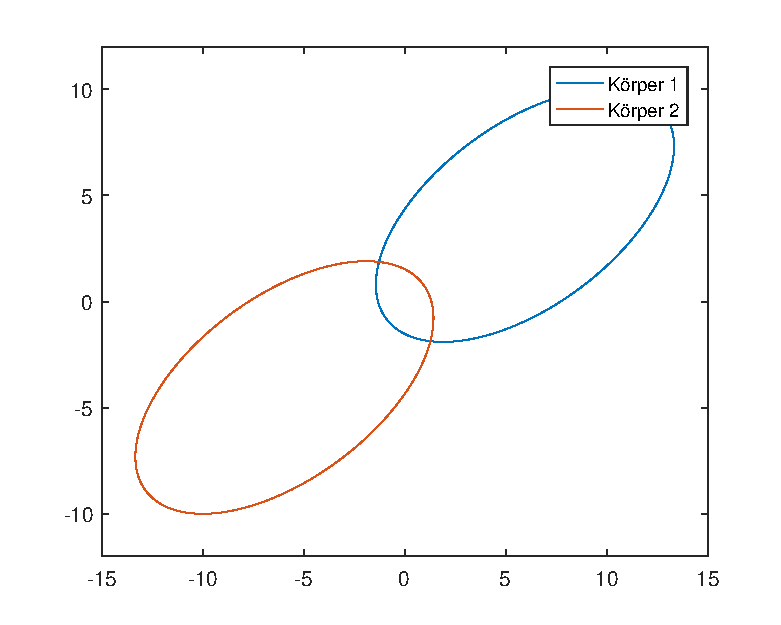
\includegraphics{schrittlaenge/images/ellipseOptimal.pdf}
\caption{Exakte L"osung: Ellipsen}
\label{image:ellipseOptimal}
\end{figure}
\begin{figure}
\centering
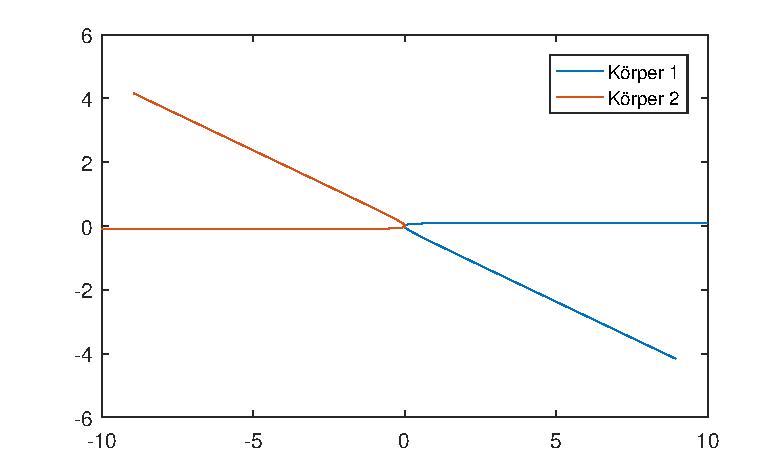
\includegraphics{schrittlaenge/images/hyperbelOptimal.pdf}
\caption{Exakte L"osung: Hyperbeln}
\label{image:hyperbelOptimal}
\end{figure}
\begin{figure}
\centering
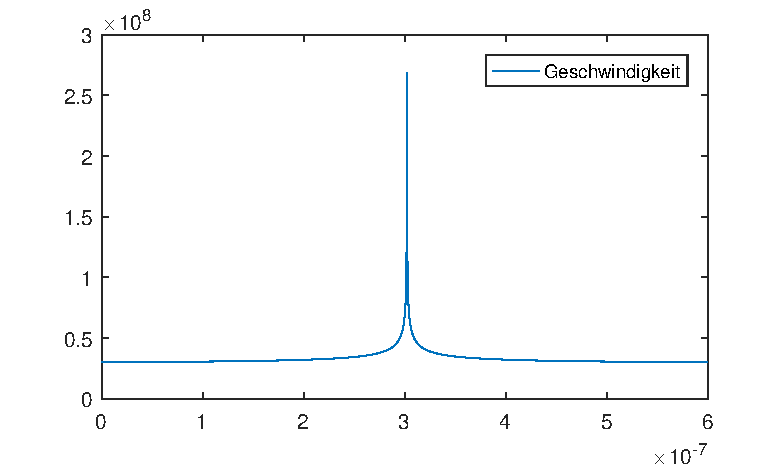
\includegraphics{schrittlaenge/images/geschwindigkeitHyperbel.pdf}
\caption{Momentane Geschwindigkeit}
\label{image:geschwindigkeitHyperbel}
\end{figure}

\section{Runge-Kutta-Schritt\label{section:schrittlaenge:runge-kutta}}
\rhead{Runge-Kutta-Verfahren}

Nun wird ein Algorithmus ben"otigt, mit dem man die Berechnung des Beispielproblems vornehmen kann.
MATLAB und viele andere Mathematikprogramme beinhalten bereits solche Algorithmen.
Ein in MATLAB weit verbreitetes Beispiel daf"ur ist der \texttt{ode45}, welcher mit einem Runge-Kutta-Verfahren f"unfter Ordnung arbeitet.
Das Problem bei Standardl"oseverfahren wie dem \texttt{ode45} ist, dass die Schrittl"ange nur in begrenztem Masse steuerbar ist. 
Darum ist es sinnvoll eine eigene Implementation des Runga-Kutta-Verfahrens zu verwenden. Der Einfachheit halber wird das Verfahren aus Abschnitt \ref{subsection:numerik:runge-kutta} verwendet. 
\begin{lstlisting}[style=MATLAB, caption=Runge-Kutta-Schritt, captionpos=b, label=code:rk4Step] 
function y = rk4Step(ode, t0, y0, h)            %ode: Problemfunktion
                                                %t0 : Anfangszeitpunkt  
                                                %y0 : Anfangsbedingung 
                                                %h  : Schrittlaenge
                                                
    hDiv2 = h / 2;                              %Schrittlaenge halbieren
    t1 = t0 + hDiv2;                            %Zeitpunkt nach halbem Schritt

    k1 = ode(t0, y0).';                         %berechnen der vier Steigungen
    k2 = ode(t1, y0 + hDiv2 * k1).';               
    k3 = ode(t1, y0 + hDiv2 * k2).';
    k4 = ode(t0 + h, y0 + h * k3).';
    
    y = y0 + h * (k1 + 2*k2 + 2*k3 + k4)./6;    %naechster Wert

end
\end{lstlisting}

Die MATLAB-Funktion \texttt{rk4Step} \ref{code:rk4Step} liefert den n"achsten Wert \texttt{y} zur"uck, welcher aus dem vorherigen Wert \texttt{y0} sowie dem vorherigen Zeitpunkt \texttt{t0} berechnet wird.
Die Zeit zwischen \texttt{y0} und \texttt{y} entspricht dabei der Schrittl"ange \texttt{h}.
Als Parameter wird die Problemfunktion \texttt{ode}, welche im aktuellen Beispiel die Funktion \texttt{planets} \ref{code:planets} ist, an die Funktion "ubergeben.
Weiter wird der Ausgangszeitpunkt \texttt{t0}, der Ausgangswert \texttt{y0} sowie die Schrittl"ange \texttt{h} mitgegeben.
 
\section{Konstante Schrittl"ange}
\rhead{Konstante Schrittl"ange}

Dank der eigenen Implementation des Runge-Kutta-Verfahrens kann nun die Schrittl"ange frei gew"ahlt werden.
So kann das Beispielproblem sehr einfach mit konstanter Schrittl"ange berechnet und die Ergebnisse verglichen werden. 
\begin{lstlisting}[style=MATLAB, caption=Konstante Schrittl"ange, captionpos=b, label=code:fixRk4] 
function [t, y] = fixRk4(ode, x, y0, h)                 
    len = ceil((x(2) - x(1)) / h + 1);              %Anzahl Schritte berechnen

    t = zeros(len, 1);                              %Speicher allozieren
    y = zeros(len, size(y0,2));

    t(1) = x(1);                                    %Anfangszeitpunkt an
                                                    %Zeitvektor zuweisen
                                                        
    y(1,:) = y0;                                    %Anfangswert an
                                                    %Loesungsvektor zuweisen
    for i = 2:len
  
        y(i,:) = rk4Step(ode, t(i-1), y(i-1,:), h); %naechster Schritt
                                                    %berechnen
        t(i) = t(i-1) + h;                             

    end
end
\end{lstlisting}

Mit der MATLAB-Funktion \texttt{fixRk4} \ref{code:fixRk4} kann nun ein Problem mit einer vorgew"ahlten Schrittl"ange gel"ost werden.
Diese Schrittl"ange bleibt "uber die gesamte Zeitspanne konstant.
Dabei wird der Funktion neben der Problemfunktion \texttt{ode} auch die Zeitspanne \texttt{x}, die Anfangsbedingunen \texttt{y0} sowie die Schrittl"ange \texttt{h} "ubergeben.
Die Zeitspanne \texttt{x} ist ein Vektor bestehend aus den zwei Komponenten Anfangszeitpunkt \texttt{x(1)} und Endzeitpunkt \texttt{x(2)}.
Die Parameter welche von der Funktion zur"uckgegeben werden, sind \texttt{t} und \texttt{y}, wobei \texttt{t} den Zeitpunkten und \texttt{y} den Werten an diesen Zeitpunkten entsprechen.

\begin{figure}
\centering
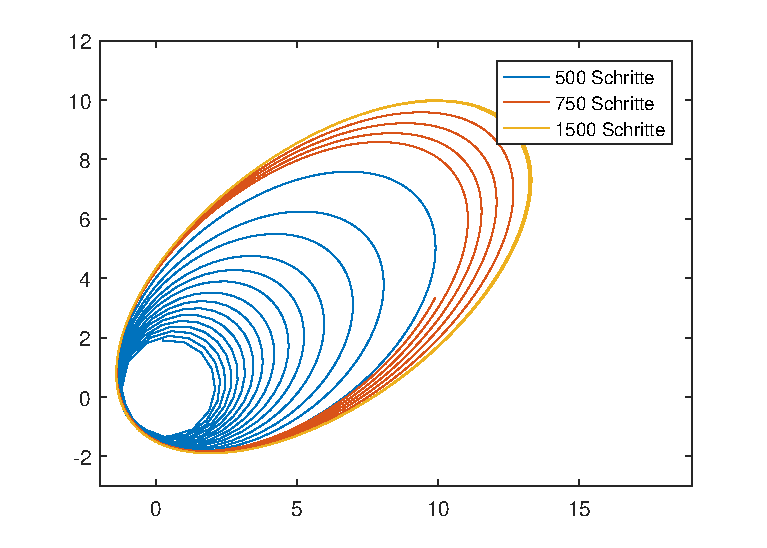
\includegraphics{schrittlaenge/images/fixStepVergleichEllipse.pdf}
\caption{Vergleich unterschiedliche Schrittl"angen: Ellipse}
\label{image:fixStepVergleichEllipse}
\end{figure}
\begin{figure}
\centering
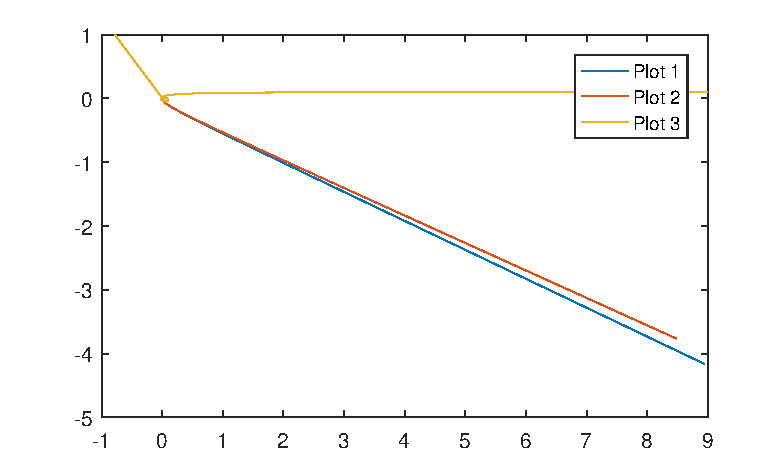
\includegraphics{schrittlaenge/images/fixStepVergleichHyperbel.pdf}
\caption{Vergleich unterschiedliche Schrittl"angen: Hyperbel}
\label{image:fixStepVergleichHyperbel}
\end{figure}
Im Bild \ref{image:fixStepVergleichEllipse} sind die Bahnen eines K"orpers, berechnet mit unterschiedlichen Schrittl"angen und darum auch unterschiedlichen Anzahl Schritten, ersichtlich.
W"urde das Problem analytisch gel"ost werden, ergäbe sich die Form einer perfekten Ellispe.
Dies ist hier vorallem bei den Kurven, welche mit weniger Schritten berechnet wurden, nicht der Fall.
Mit ver"anderten Anfangsbedingungen kann aus der Ellipse eine Hyperbel werden.
Der Versatz der beiden K"orper in Richtung der y-Achse wurde verkleinert, so dass es fast zu einer Kollision kommt. 
Dies ist in Bild \ref{image:fixStepVergleichHyperbel} erkennbar.

Bei einer Fastkollision ist die Richtungs"anderung an einer Stelle sehr gross, davor und danach treten nur sehr kleine Kr"ummungen auf.
Diese grosse Kr"ummung ist ein entscheidender Punkt in der Berechnung der Gesamtkurve, denn ist die Abweichung dort zu gross, stimmt der ganze folgende Verlauf der Kurve nicht.
Aus diesem Grund ist eine sehr kleine Schrittl"ange unabdingbar.
F"ur eine korrekte Berechnung sind deshalb sehr viele Schritte n"otig, wie Tabelle \ref{table:fixStepVergleichHyperbel} zeigt.
\begin{table}
\centering
\begin{tabular}{|l|r|r|}
\hline
Plot \# & Anzahl Schritte & Schrittl"ange\\ \hline
1 & 60'000 & $10^{-11}$\\ \hline
2 & 20'000 & $3 \cdot 10^{-11}$\\ \hline
3 & 6'000 & $10^{-10}$\\ \hline
\end{tabular}
\caption{Vergleich Schrittl"ange: Hyperbel}
\label{table:fixStepVergleichHyperbel}
\end{table}
\begin{figure}
\centering
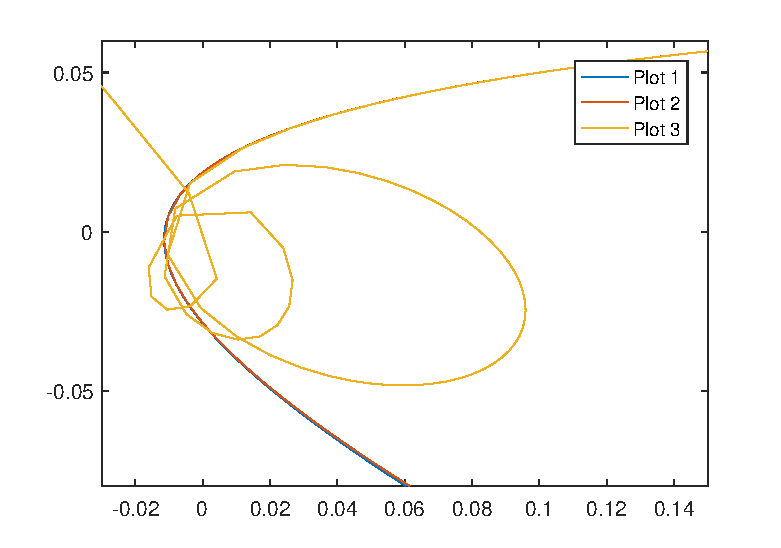
\includegraphics{schrittlaenge/images/fixStepVergleichHyperbelZoom.pdf}
\caption{Vergr"osserter Ausschnitt von Bild \ref{image:fixStepVergleichHyperbel}}
\label{image:fixStepVergleichHyperbelZoom}
\end{figure}

Das Bild \ref{image:fixStepVergleichHyperbelZoom} zeigt einen vergr"osserten Ausschnitt in der Umgebung der Fastkollision.
Hierbei muss beachtet werden, dass nur die rechte der zwei punktsymmetrischen Bahnen dargestellt wird.
Beim Begutachten von Bild \ref{image:fixStepVergleichHyperbel} wird klar, warum eine Schrittl"angensteuerung von grosser Bedeutung ist.
Denn so k"onnen die mehr oder weniger geraden Strecken mit einer grossen Schrittl"ange schnell berechnet und damit einen Grossteil der Rechenzeit f"ur die kritische Stelle aufgewendet werden.

\section{Variable Schrittl"ange}
\rhead{Variable Schrittl"ange}

Um die Schrittl"ange adaptiv gestalten zu k"onnen, wird ein Kriterium ben"otigt, welches eine Aussage dar"uber macht, wie gross die Schrittl"ange sein sollte.
Je gr"osser die Kr"ummung der Kurve, umso kleiner sollte die Schrittl"ange sein.
Die Schwierigkeit dabei ist, dass weder die aktuelle Kr"ummung noch der zuk"unftige Verlauf der Kurve bekannt ist.
Weiter ist es diffizil, einer bestimmten Kr"ummung die entsprechende Dimension der Schrittl"ange zuzuordnen.
Deshalb wurde dieser L"osungsansatz verworfen.

Eine weitere Strategie ist, den n"achsten Schritt mit zwei verschiedenen Verfahren zu berechnen, um anschliessend die beiden L"osungen zu vergleichen.
"Uberschreitet die Differenz der L"osungen eine vorgegebene Toleranz, wird die Schrittl"ange halbiert und die Berechnung erneut durchgef"uhrt.
Damit ergibt sich aber folgendes Problem: Die Schrittl"ange wird zwar verkleinert sobald die Toleranz nicht eingehalten wird, aber sie wird nie vergrössert.
Aus diesem Grund wird die Schrittl"ange vor jedem Schritt zun"achst um den Faktor $\sqrt{2}$ vergr"ossert. 
Damit nur ein Verfahren implementiert werden muss, wird folgender Trick angewendet: 
Das erste Verfahren entspricht dem Runge-Kutta-Verfahren, welches im Abschnitt \ref{section:schrittlaenge:runge-kutta} erw"ahnt wird.
Beim Zweiten wird das erste Verfahren mit halbierter Schrittl"ange zweimal angewendet. 
\begin{lstlisting}[style=MATLAB, caption=Variable Schrittl"ange, captionpos=b, label=code:myOde] 
function [t, y] = myOde(ode, x, y0, h0, tol)
    
    y = [y0; rk4Step(ode, x(1), y0, h0)]; 
    t = [x(1); x(1) + h0];
    
    while t(end) < x(2)
        
        hBig = h0 * sqrt(2);
        hSmall = hBig / 2;
        
        yLast = y(end,:);
        tLast = t(end);
        
        % naechster Schritt berechnen
        yBig = rk4Step(ode, tLast, yLast, hBig);
        ySmall1 = rk4Step(ode, tLast, yLast, hSmall);
        ySmall2 = rk4Step(ode, tLast + hSmall, ySmall1, hSmall);
        
        % Fehlerberechnung
        absError = abs(yBig - ySmall2);
        change = abs(ySmall2 - yLast);
        
        relError = absError ./ change;
        
        if max(relError) > tol
            h0 = hSmall;
            y = [y; ySmall1];
            t = [t; tLast + h0];
        else
            h0 = hBig;
            y = [y; yBig]; 
            t = [t; tLast + h0];           
        end
         
    end
end
\end{lstlisting}

Im Codebeispiel \ref{code:myOde} wird statt der konstanten Schrittl"ange \texttt{h} nur die Anfangsschrittl"ange \texttt{h0}, sowie zus"atzlich die Toleranz \texttt{tol}, "ubergeben.
Zuerst wird die Schrittl"ange \texttt{h0} vergr"ossert.
Dies entspricht im Code \texttt{hBig}.
Anschliessend wird die erste L"osung \texttt{yBig} mit dem Runge-Kutta-Verfahren berechnet.
Mit der halben Schrittl"ange \texttt{hSmall} werden nun hintereinander die L"osungen \texttt{ySmall1} und \texttt{ySmall2} mit dem selben Verfahren berechnet.
Direkt danach wird der relative Fehler berechnet.
Ist dieser gr"osser als die spezifizierte Toleranz, wird als die neue Schrittl"ange \texttt{hSmall} gew"ahlt und die erste L"osung mit dieser Schrittl"ange verwendet.
Ansonsten wird der grosse Schritt verwendet.

\begin{figure}
\centering
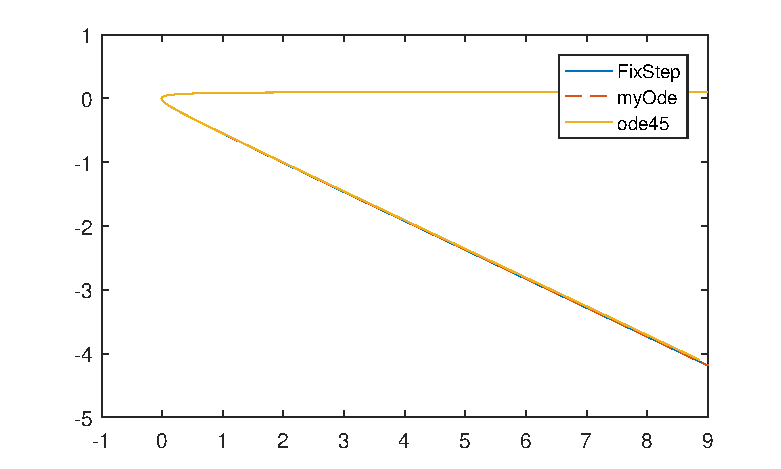
\includegraphics{schrittlaenge/images/vergleichVerfahren.pdf}
\caption{Vergleich unterschiedliche Verfahren}
\label{image:vergleichVerfahren}
\end{figure}
\begin{table}
\centering
\begin{tabular}{|l|r|}
\hline
Verfahren & Anzahl Schritte\\ \hline
fixStep & 60'000\\ \hline
myOde & 128\\ \hline
ode45 & 197\\ \hline
\end{tabular}
\caption{Vergleich Verfahren}
\label{table:vergleichVerfahren}
\end{table}
Mit dem entwickelten Algorithmus kann die Anzahl Schritte und somit der Rechenaufwand massgeblich reduziert werden.
Dies ist in Bild \ref{image:vergleichVerfahren} und Tabelle \ref{table:vergleichVerfahren} zu sehen.
Zum Vergleich wurde auch der Standard-Solver \texttt{ode45} aus MATLAB herangezogen.
Der entwickelte Algorithmus \texttt{myOde} braucht weniger Schritte um eine bessere L"osungskurve als der \texttt{ode45} zu erhalten.
Allerdings kann keine Aussage dar"uber gemacht werden, ob der schlussendliche Rechenaufwand effektiv geringer war.
Dies, weil die Funktionsweise des \texttt{ode45} nicht n"aher untersucht wurde.
\begin{figure}
\centering
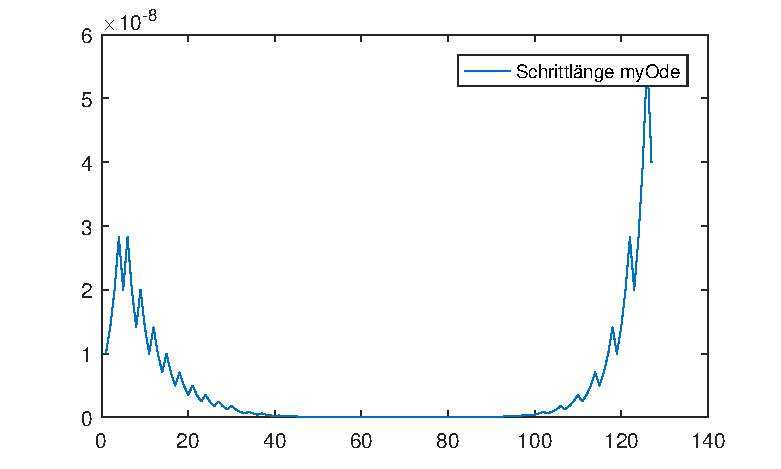
\includegraphics{schrittlaenge/images/verlaufSchrittlaenge.pdf}
\caption{Verlauf der Schrittl"ange}
\label{image:verlaufSchrittlaenge}
\end{figure}
In Bild \ref{image:verlaufSchrittlaenge} kann der Verlauf der Schrittl"ange, welcher sich zur Berechnung der L"osungskurve mit \texttt{myOde} ergeben hat, herausgelesen werden.
Eindr"ucklich ist, dass der Grossteil der Schritte sehr klein ist.
Dies weil etwa 80\% der Schritte zur Berechnung der kritischen Stelle aufgewendet werden.

\section{Schwierigkeiten}
\rhead{Schwierigkeiten}

Beim Konfigurieren eines Algorithmus zur Schrittl"angensteuerung treten verschiedene Schwierigkeiten auf.
Die offensichtichste davon ist die Wahl der Anfangsschrittl"ange.
Da die Gr"ossenordnung des Problems unbekannt ist, wird es unm"oglich, eine vern"unftige Anfangsschrittl"ange mitzugeben.
Wird sie zu gross gew"ahlt, kann es sein, dass eine kritische Stelle der Kurve verpasst wird.
Wird sie zu klein gew"ahlt, geht es unter Umst"anden sehr lange bis der Algorithmus die Schrittl"ange dem Problem angepasst hat.

Eine weitere Schwierigkeit ist die Wahl der Toleranz.
Je gr"osser diese gew"ahlt wird, desto kleiner wird der Rechenaufwand, allerdings leidet die Genauigkeit darunter.
Darum muss je nach Problemstellung ein Kompromiss zwischen Rechenaufwand und Genauigkeit gefunden werden.
Dies kann in Bild \ref{image:myOdeToleranz}, sowie in Tabelle \ref{table:myOdeToleranz} beobachtet werden.

Um diese Parameter richtig einstellen zu k"onnen, ist es substantiell, dass schon vor der Berechnung eine ungef"ahre Vorstellung des Problems vorhanden ist.
Weil die Algorithmen nicht unfehlbar und zum Teil sogar recht ungenau sind, kann sonst nicht abgesch"atzt werden, ob eine L"osungskurve plausibel ist oder nicht.
\begin{figure}
\centering
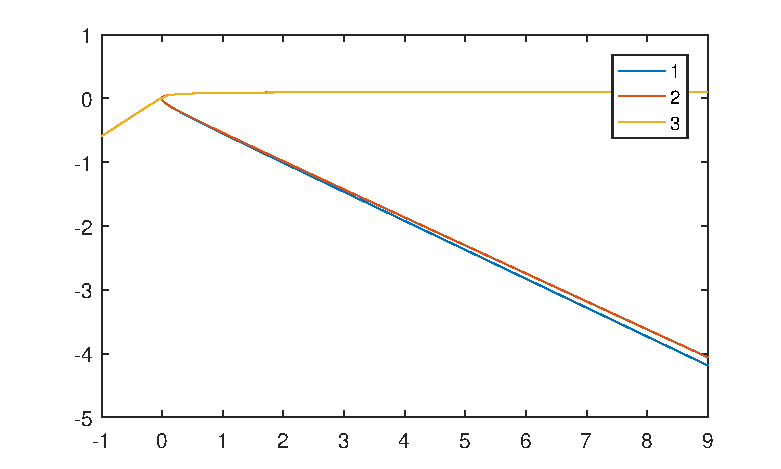
\includegraphics{schrittlaenge/images/myOdeToleranz.pdf}
\caption{myOde mit verschiedenen Toleranzen}
\label{image:myOdeToleranz}
\end{figure}
\begin{table}
\centering
\begin{tabular}{|l|l|r|}
\hline
Plot & Toleranz & Anzahl Schritte\\ \hline
1 & 0.0001 & 128\\ \hline
2 & 0.001 & 69\\ \hline
3 & 0.01 & 33\\ \hline
\end{tabular}
\caption{myOde mit verschiedenen Toleranzen}
\label{table:myOdeToleranz}
\end{table}

Zus"atzlich zum vorgestellten Algorithmus \texttt{myOde} wurde noch ein anderer Ansatz verfolgt.
Die Idee hinter diesem war, die Kr"ummung der schon berechneten Kurve zu analysieren und daraus ein R"uckschluss auf die zuk"unftige Schrittl"ange zu treffen.
So sollte die Schrittl"ange kleiner werden, wenn die Kurve enger wird und umgekehrt.
Das Problem dieser Variante ist, das es kein Anhaltspunkt gibt, welcher aussagen kann, ob die Schrittl"ange schon genug klein oder gen"ugend gross ist.
So werden bei einer sich verengenden Kurve die Schritte beliebig klein. Dies kann abgefangen werden, wenn zum Beispiel eine minimale Schrittweite als Parameter definiert wird.
Jetzt tritt aber ein neues Problem auf: Wie gross soll dieser Parameter gew"ahlt werden, dass sich trotzdem eine L"osungskurve mit einer zufriedenstellenden Genauigkeit ergibt?
Aufgrund dieser Unannehmlichkeiten wurde der Ansatz nicht weiter verfolgt und der Schwerpunkt auf die Verfeinerung des besseren \texttt{myOde} Algorithmus gesetzt.  

\end{refsection}

